\documentclass{beamer}[10]


%
% macro
%
\usepackage{pgf}
\usepackage[english]{babel}
\usepackage[utf8]{inputenc} % use unicode chars
\usepackage{lmodern}% http://ctan.org/pkg/lm
\usepackage{beamerthemesplit}
\usepackage{graphics,epsfig,subfigure}
\usepackage{url}
\usepackage{srcltx}
\usepackage{hyperref}
\usepackage[mathescape,escapeinside=||]{minted}
\usepackage{import}
\usepackage{mathtools}
\usepackage{amsmath}
\usepackage{color}
%\usepackage[beamer]{hf-tikz}
\usepackage{xfrac}
\usepackage{makeidx}
\usepackage{multicol}

%\showboxdepth=5
%\showboxbreadth=5

% Slides in 16:9
\usepackage[orientation=landscape,size=custom,width=16,height=9,scale=0.5,debug]{beamerposter} 

%
% Macros
%
\definecolor{darkred}{rgb}{0.55, 0.0, 0.0}
\definecolor{light-gray}{gray}{.80}
\definecolor{light-yellow}{rgb}{255,255,153}
\definecolor{alizarin}{rgb}{0.82, 0.1, 0.26}
% colorized font
\newcommand{\red}[1] {{\color{red} #1}}
\newcommand{\darkred}[1] {{\color{darkred} #1}}
\newcommand{\blue}[1] {{\color{blue} #1}}
\newcommand{\green}[1] {{\color{green} #1}}
\newcommand{\gray}[1] {{\color{gray} #1}}
\newcommand{\grey}[1] {{\color{gray} #1}}

\newcommand{\hearts} {\red{$\heartsuit$}}
\newcommand{\diamonds} {\red{$\diamondsuit$}}
\newcommand{\spades} {$\spadesuit$}
\newcommand{\clubs} {$\clubsuit$}
\newcommand{\pyoptional}[1]{\diamonds #1 \diamonds}

\newcommand{\deltasum}[1]{\sum (#1 - \bar{#1})}
\newcommand{\deltasumsq}[1]{\sum (#1 - \bar{#1})^{2}}

%
% Take care of the newline after \frametitle
%
\newenvironment{pyframe}[1]
{\begin{frame}[fragile,environment=pyframe]\frametitle{#1}
 
}
{\end{frame}}


% environments
\newminted{py}{mathescape,escapeinside=||}% 
\newminted{bash}{mathescape,escapeinside=||}%

% python highlights: module, method
\newcommand{\pymodule}[1]{\darkred{\textbf{#1}}}
\newcommand{\pyfunction}[1]{\textit{#1}}
\newcommand{\keyword}[1]{\texttt{#1}}
\newcommand{\pyver}[1]{\colorbox{yellow}{#1}}
\newcommand{\typeonly}[1]{\colorbox{green}{#1}}
\newcommand{\pyvers}[1]{\raisebox{0em}{\colorbox{yellow}{#1}}}
\newcommand{\code}[1] { \texttt{#1} }

% special symbils
\newcommand{\mymapsto}{\operatornamewithlimits{\longmapsto}}

\makeatletter
\newcommand{\xMapsto}[2][]{\ext@arrow 0599{\Mapstofill@}{#1}{#2}}
\def\Mapstofill@{\arrowfill@{\Mapstochar\Relbar}\Relbar\Rightarrow}
\makeatother




%
% style
%

\setbeamercovered{transparent}
\mode<presentation>

%\geometry{top=5pt, margin=5pt}
%The outertheme defines the head and the footline of each slide
% \setbeamercolor{block title}{bg=orange}
% \useinnertheme{circles}
% \useoutertheme{split}
%\beamertemplatenavigationsymbolsempty

%\usetheme[numbers,totalnumber,compress,sidebarshades]{Babel}
\setbeamertemplate{headline}{
 \leavevmode%
  \hbox{%
%,bb=0 0 5cm 2cm
    \hspace{5pt}\includegraphics[height=1.2cm]{logo.eps}
    \hspace{240pt}\includegraphics[height=1.2cm]{logo.eps}
    }
}
\setbeamertemplate{footline}{
\noindent\textbf{\hspace{5pt}\insertsection \insertsubsection\hfill}\textbf{\hfill{\color{gray}\insertshortauthor}\hfill}\textbf{\hfill }
   % \textline[t]{ \insertsection  \insertsubsection}{\gray{\insertshortauthor}}{right}
}
%\useinnertheme[shadow=false]{rounded}
% frametitle
\setbeamertemplate{frametitle}[default][center]
\setbeamercolor*{frametitle}{bg=white,fg=gray,parent=palette primary}
\setbeamerfont{frametitle}{series=\bfseries,size={\fontsize{16}{8}}}
% table of contents
\setbeamercolor{section in toc}{fg=black} % series=\bfseries,size={\fontsize{16}{8}}}
%\setbeamercolor{section/subsection in toc}{fg=black}
%\setbeamercolor{subsection in toc}{fg=black}
%\setbeamerfont{section in toc}{fg=black} % series=\bfseries,size={\fontsize{16}{8}}}
%\setbeamerfont{section/subsection in toc}{fg=black}
%\setbeamerfont{subsection in toc}{fg=black}

%title
\setbeamercolor{title}{fg=black,bg=white}
\setbeamerfont{title}{series=\bfseries,size={\fontsize{24.88}{32}}}
%subtitle
\setbeamercolor{subtitle}{fg=gray}
\setbeamerfont{subtitle}{series=\bfseries,size={\fontsize{14}{}}}
%titlepage
\setbeamertemplate{title page}[default][center]
% bullets
\setbeamercolor{itemize item}{fg=gray}
\setbeamertemplate{itemize items}[circle]
\setbeamercolor{itemize item}{fg=light-gray}
\setbeamercolor{itemize items}{fg=light-gray}
% enumerations
\setbeamercolor{enumerate item}{fg=black}
\setbeamercolor{local structure}{fg=black}

%
% increase itemize spacing
%
%\newlength{\wideitemsep}
%\setlength{\wideitemsep}{\itemsep}
%\addtolength{\wideitemsep}{14pt}
%\let\olditem\item
%\renewcommand{\item}{\setlength{\itemsep}{\wideitemsep}\olditem}

  % \usecolortheme[named=orange]{structure}
  % \useinnertheme{circles}
  % \usefonttheme[onlymath]{serif}
\setbeamercovered{transparent}
  % \setbeamertemplate{blocks}[rounded][shadow=true]

\makeindex


% Apply DRAFT watermark
\usepackage{draftwatermark}
\setbeamercolor{background canvas}{bg=}%transparent canvas


\title{Scaling MySQL with Python}
%\subtitle{EuroPython 2015, $21-27^{th}$ July - Bilbao}
\subtitle{draft2}
\author{Roberto Polli - \href{mailto:roberto.polli@par-tec.it}{roberto.polli@par-tec.it}}
\date{21-27 July 2015}
\institute{Par-Tec Spa - Rome Operation Unit\\
    P.zza S. Benedetto da Norcia, 33\\
    00040, Pomezia \(RM\) - www.par-tec.it
    }%

%
%
\begin{document}

%% cover
\frame{\titlepage 
\vspace{-0.5cm}
}

%% agenda
%\iffalse
\frame{\frametitle{Agenda}
\tiny
\tableofcontents%[pausesection]
}
%\fi

%% Starting doc
\section{Intro}
\begin{pyframe}{Who? What? Why?}
\begin{itemize}

\item Manage, replicate, scale MySQL databases with python
\\

\item Roberto Polli - Solutions Architect @ par-tec.it. Loves writing in C,
Java and Python. Red Hat Certified Engineer and Virtualization
Administrator.
\\
\\
\item Par-Tec – Proud sponsor of this talk ;) Contributes to various FLOSS. \\
Provides expertise in IT Infrastructure \& Services and \\ Business Intelligence
solutions + Vertical Applications for the financial market.

\end{itemize}
\end{pyframe}

\begin{pyframe}{Agenda}
\begin{itemize}
\item MySQL architecture
\item Getting informations
\item Comparing databases
\item Replication 2.0 aka GTID
\item Fabric: scaling \& sharding for the masses
%\item modules: \pymodule{scipy, matplotlib}
\end{itemize}
\end{pyframe}


\section{Architecture}
\begin{pyframe}{MySQL Architecture}
\begin{itemize}
\item MySQL is not only SQL
% Query parser vs engine store
\item Architecture of a database
% query parser, cache, transaction log, MVCC
% http://www.oracle.com/technetwork/articles/javase/figure2-large-145676.jpg
\item MVCC
\item Replication
\item Consistency is here to stay
%
\end{itemize}
\end{pyframe}


\begin{pyframe}{MySQL Architecture}
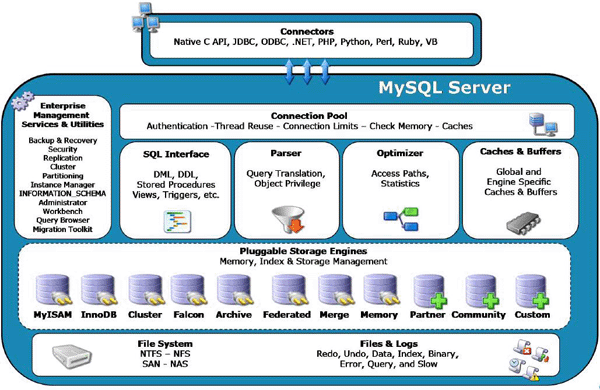
\includegraphics[height=5.5cm]{images/mysql-architecture.pdf}
{\large
    \begin{center}
    It's a lot of stuff
    \end{center}
}
\end{pyframe}


\begin{pyframe}{MySQL Architecture}
% Map in the figure every task
We should manage and monitor
    \begin{itemize}
    \item Database size: Tables, Indexes, Binary Logs
    \item Replication inconsistencies
    \item Failover
    \end{itemize}
Simplify please!
\end{pyframe}



\section{Utilities}
\begin{pyframe}{Get the code}
    % https://dev.mysql.com/get/Downloads/MySQLGUITools/mysql-utilities-1.6.1.tar.gz
    \begin{bashcode}
    # wget http://bit.ly/1CxNuZe
    # tar xf mysql-utilities-1.6.1.tar.gz
    # python setup.py install
    \end{bashcode}

\iffalse
            or
        % # yum -y install https://dev.mysql.com/get/mysql-community-release-el7-5.noarch.rpm
        \begin{bashcode}
        # Fedora / RHEL / Centos
        yum -y install http://bit.ly/1yhSViu # MySQL Community repo
        yum -y install mysql-utilites
        # Ubuntu
        apt-get -y install mysql-utilites
        \end{bashcode}

\fi

\end{pyframe}


\begin{pyframe}{Utilities}
Drivers
\begin{pycode}
    # mysql.connector.django.introspection
    if django.VERSION >= (1, 6):
        from django.db.backends import FieldInfo
        if django.VERSION >= (1, 7):
            ...
\end{pycode}
Utilities
\begin{pycode}
    # mysql.utilities.common.replication
    if master_innodb_stats != slave_innodb_stats:
        if not pedantic:
            errors.append("WARNING: Innodb settings differ "
                          "between master and slave.")
    ...
\end{pycode}
Fabric Orchestrator
\end{pyframe}

\begin{pyframe}{Single Entrypoint: mysqluc}
\begin{columns}
\column[t]{.5\linewidth}
    Start with \code{mysqluc}
    \begin{itemize}
    \item An entrypoint for all utilities
    \item Contextual help
    \item TAB completion
    \end{itemize}

\column[t]{.5\linewidth}
    Or call each method separately
    \begin{itemize}
    \item mysqldiskusage
    \item mysqldbexport / mysqldbimport
    \item mysqlcompare / mysqldiff
    \item ...
    \item mysqlfailover
    \end{itemize}
\end{columns}
\end{pyframe}


\begin{pyframe}{Syntax}
Define one or more server credentials in the encrypted \code{~/.mylogin.cnf}\\ \\
\begin{bashcode}
    mysql_config_editor set
        --login-path=client # default used by mysql
        --host=localhost --user=localuser
        --password # (prompted)

    mysql # by default uses --login-path=client
\end{bashcode}

A SERVER is identified by the string
\begin{bashcode}
    user:password@hostname[:port] # default port 3306
\end{bashcode}
or
\begin{bashcode}
    login-path
\end{bashcode}
We will use the example \href{http://dev.mysql.com/doc/index-other.html}
{sakila database} throughout the slide.

\end{pyframe}


\subsection{Administration}
\begin{pyframe}{Disk usage}
A single command to show all disk usage infos (excluded system logs)

\begin{bashcode}
$ mysqldiskusage --all --server=$SERVER %% |grep -- =
...
Total database disk usage = 7601892 bytes or 7.25 MB
...
Current binary log file = s-1-bin.000009
...
Total size of binary logs = 231 bytes
\end{bashcode}
\end{pyframe}


%
% Exporting and Importing
%
\subsection{Export/Import}

\begin{pyframe}{Export - I}
Forget mysqldump and use the following
command for a consistent $logical$ backup.
\begin{bashcode}
$ mysqldbexport > data.sql \
    --server=$SERVER
    --all
\end{bashcode}
% --export=master --rpl=master --rpl-user=rpl:rpl
\\ \\
{
\large
To backup big databases, use InnoDB engine and an InnoDB backup tool!
}
\end{pyframe}


\begin{pyframe}{Import - I}
Then import the dump with
\begin{bashcode}
$ mysqldbimport --server=$SERVER \
    data.sql
\end{bashcode}
To provision a new slave we'll use a similar
procedure with some variants.
\end{pyframe}


%
% Comparing
%
\subsection{Comparison}
\begin{pyframe}{Comparing databases - I}
To compare databases between servers, use
\begin{bashcode}
#mysqldbcompare \
    --server1=$MASTER \
    --server2=$SLAVE \
    sakila -a --difftype=SQL \
    --show-reverse --quiet
\end{bashcode}

\end{pyframe}


\begin{pyframe}{Comparing databases - II}
Create the statemets to fix the differences!
\begin{bashcode}
mysqldiff \
    --server1=$MASTER --server2=$SLAVE \
    sakila:sakila \ # db name on master:slave
    --changes-for=server2
\end{bashcode}
\end{pyframe}


%
% replication
%
\subsection{Replication}
\begin{pyframe}{Configuring replication}
Replication is $asynchronous$ and the agreements are configured on the slave only.

\begin{columns}[t]
\column[t]{.5\linewidth}
    {\large Master}
    \begin{itemize}
    \item produces a changelog named binlog;
    \item grants access to a $replica$ user;
    \item may track slave-updates.
    \end{itemize}
    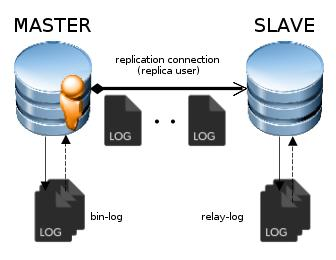
\includegraphics[height=3cm]{images/mysql-replica-hla.jpg}
\column[t]{.5\linewidth}
    {\large Slave}
    \begin{itemize}
    \item connects to the master with the $replica$ user
    \item retireves the binlog and applies the changes;
    \item \code{START SLAVE;}
    \end{itemize}
\end{columns}
\end{pyframe}


\begin{pyframe}{Replication 2.0}
MySQL 5.6+ replication is based on Global Transaction ID
\begin{itemize}
\item each server has a unique UUID \\
eg: \code{3E11FA47-71CA-11E1-9E33-C80AA9429562}
\\ \\
\item every TransactionID becomes global\\
\begin{pycode*}{escapeinside=||}
eg: 3E11FA47-71CA-11E1-9E33-C80AA9429562:|32|
\end{pycode*}
\end{itemize}
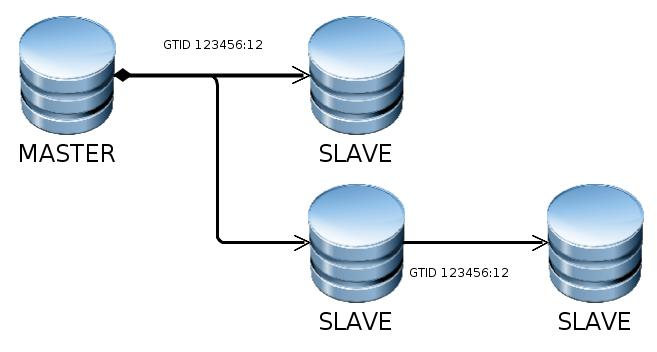
\includegraphics[height=3cm]{images/mysql-propagate-gtid.jpg}

{\large
    If binlog have been purged, you need to import the
master database first!
}

\end{pyframe}



\begin{pyframe}{Configuring replication}
mysqlreplicate takes care of
\begin{itemize}
\item provisioning the replica user on the master;
\item configure the slave to point to the master;
\item start loading the first available transaction in bin-logs;
\end{itemize}

\begin{bashcode}
    mysqlreplicate  --master=$MASTER --slave=$SLAVE \
     --rpl-user=repl:rpass \
     -b

    # master on 192.168.1.1: ... connected.
    # slave on 192.168.1.2: ... connected.
    # Checking for binary logging on master...
    # Setting up replication...
    # ...done.
\end{bashcode}
\end{pyframe}


\begin{pyframe}{Configuring replication - II}
mysqldbexport can be used to provision a new slave!
\begin{itemize}
%\item check that replica user is provisioned on the master;
\item issue a \code{RESET MASTER;};
\item add \code{--rpl=master} to store replica infos in the sql;
\end{itemize}

\begin{columns}
\column[t]{.5\linewidth}

\begin{bashcode}
# pre-import.sql
-- ignore previous changes
-- and trust the backup
STOP SLAVE;
RESET MASTER;
\end{bashcode}

\column[t]{.5\linewidth}
\begin{pycode}
$ mysqldbexport > data.sql \
 --server=$MASTER \
 --rpl-user=repl:rpass \
 --export=both \
 --rpl=master --all

\end{pycode}
\end{columns}

\end{pyframe}

%mysql $SLAVE < pre-import.sql
%mysqldbimport --server=$SLAVE \
% data.sql


\begin{pyframe}{Discovering replication}
\begin{bashcode}
$ mysqlrplshow --master=$MASTER \
    --discover-slaves-login=root:root
# master on s-1.docker: ... connected.
# |Finding slaves| for master: s-1.docker:3306
# Replication Topology Graph
s-1.docker:3306 (MASTER)
   |
   +--- s-3.docker:3306 - (SLAVE)
   |
   +--- s-4.docker:3306 - (SLAVE)
\end{bashcode}
\end{pyframe}



%
% Failover
%

\section{Failover}
\begin{pyframe}{Failover Basics}
A replicated infrastructure can be made Higly Available.
\begin{columns}

\column{.4\linewidth}
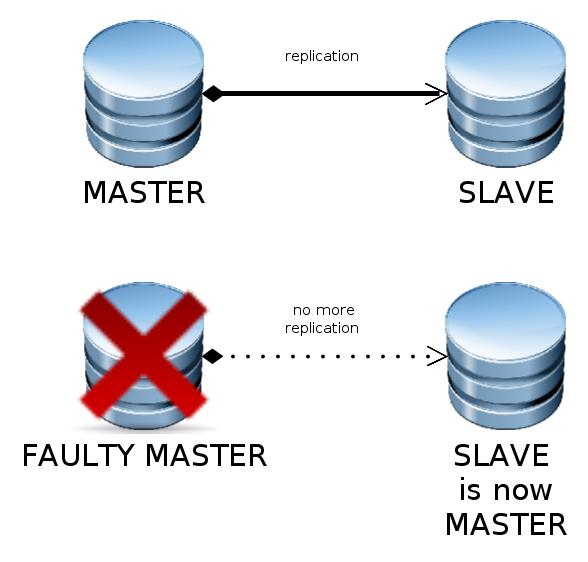
\includegraphics[height=4cm]{images/mysql-promote-slave.jpg}

\column{.4\linewidth}%
In case of fault you should:
 \begin{itemize}
 \item $promove$ your slave!
 \item reconfigure the others to point there
 \item disable the master
 \item eventually switch the ip-address
 \end{itemize}

\end{columns}
\end{pyframe}

\begin{pyframe}{Failover - I}
mysqlfailover takes care of that, and can even discover your
replication topology!

\begin{bashcode}
$ mysqlfailover --master=$MASTER \
    --discover-slaves-login=root:password \
    --candidates=$SLAVE1,$SLAVE2 \
    --exec-before=/pre-fail.sh \
    --exec-after=/post-fail.sh
\end{bashcode}
{\large
    mysqlfailover supports a lot of parameters!
    Read them carefully and test thoroughly your
    solution
    }
\end{pyframe}


\begin{pyframe}{Failover - II}
Run mysqlfailover on an existing infrastructure!
\begin{bashcode}
$ mysqlfailover --master=$MASTER \
 --discover-slaves-login=root:root
# Discovering slaves for master at s-1.docker:3306
# Discovering slave at s-3.docker:3306
# Found slave: s-3.docker:3306
# Discovering slave at s-4.docker:3306
# Found slave: s-4.docker:3306
# Checking privileges.
...
\end{bashcode}
\end{pyframe}

\begin{pyframe}{Failover - III}
Run mysqlfailover on an existing infrastructure!
\iffalse
Master Information
------------------
Binary Log File  Position  Binlog_Do_DB  Binlog_Ignore_DB
s-1-bin.000009   231

GTID Executed Set
f01a69cd-df69-11e4-b908-0242ac110009:1-3 [...]
\fi
\begin{bashcode}
MySQL Replication Failover Utility
Failover Mode = auto     Next Interval = Sun Apr 12 14:32:40 2015
...
Replication Health Status
+-------------+-------+---------+--------+------------+---------+
| host        | port  | role    | state  | gtid_mode  | health  |
+-------------+-------+---------+--------+------------+---------+
| s-1.docker  | 3306  | MASTER  | UP     | ON         | OK      |
| s-3.docker  | 3306  | SLAVE   | UP     | ON         | OK      |
| s-4.docker  | 3306  | SLAVE   | UP     | ON         | OK      |
+-------------+-------+---------+--------+------------+---------+
\end{bashcode}
\end{pyframe}



%
% Fabric
%
\begin{pyframe}{Fabric - I}
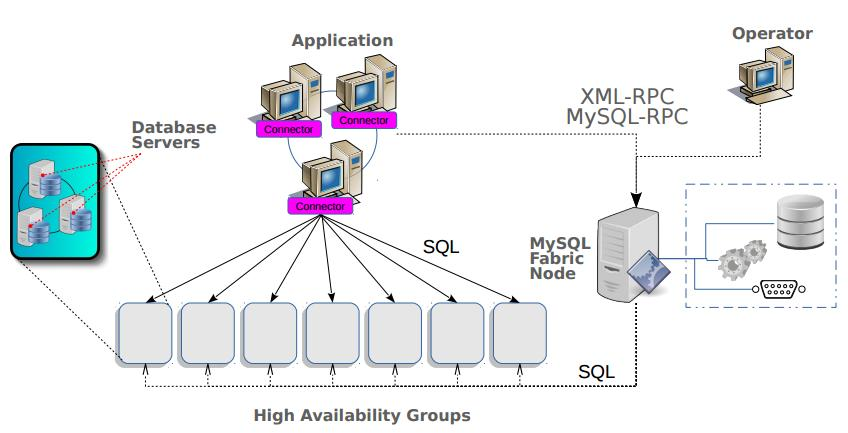
\includegraphics[height=6.6cm,width=12cm]{images/mysql-fabric-hla.jpg}
Fabric is a python framework for managing, replicating, sharding and scaling mysql clusters.
\begin{itemize}
\item tie servers in high availability groups
\item configure single-master replication topologies
\item monitor failures
\item proxy for rw/split and sharding
\end{itemize}
\end{pyframe}
%http://mysqlmusings.blogspot.it/2013/10/mysql-fabric-high-availability-groups.html


\begin{pyframe}{Fabric HLA - II}
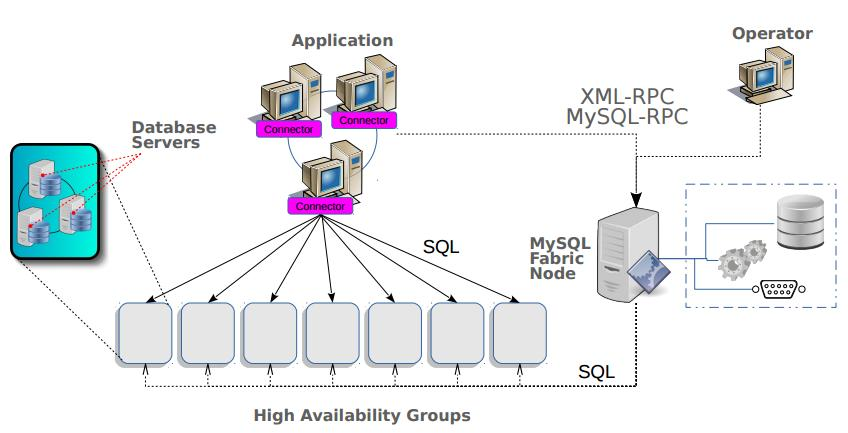
\includegraphics[height=6.6cm,width=12cm]{images/mysql-fabric-hla.jpg}
\end{pyframe}


\begin{pyframe}{Fabric Setup}
Configure \code{/etc/mysql/fabric.cfg} setting, then setup
\begin{bashcode}
# Create fabric database and
# configure endpoint properties
mysqlfabric manage setup --param=storage.user=fabric

# Startup and check if ok
mysqlfabric manage start
mysqlfabric manage ping
\end{bashcode}
\end{pyframe}


\begin{pyframe}{Fabric Groups - create\, add}
Create an High Availability group and add one or more servers
\begin{bashcode}
# add servers to fabric
mysqlfabric group create $HA
mysqlfabric group add $HA $SERVER1
...
mysqlfabric group add $HA $SERVERX
\end{bashcode}
\end{pyframe}


\begin{pyframe}{Fabric Groups - lookup}
Show groups
\begin{bashcode}
[root@fabric /]# mysqlfabric group lookup_groups
Fabric UUID:  5ca1ab1e-a007-feed-f00d-cab3fe13249e
Time-To-Live: 1

group_id description failure_detector master_uuid
-------- ----------- ---------------- -----------
      ha        None                1 f0ce9615...

\end{bashcode}
\end{pyframe}

\begin{pyframe}{Fabric Groups - promote, activate}
Now start the game
\begin{bashcode}
# Set one server as master...
$ mysqlfabric group \
    promote $HA \
     --slave_id f0ce9615-df69-11e4-b909-0242ac11000a

# .. and enable monitoring and failover
$ mysqlfabric group activate $HA
\end{bashcode}
\end{pyframe}


\begin{pyframe}{Fabric Groups - health}
Use hea
\begin{bashcode}

# and check if the group is fine
$ mysqlfabric group heath $HA
       uuid is_alive    status ... io_error sql_error
----------- -------- --------- --- -------- ---------
da42f6b1...        1 SECONDARY        False     False
f0ce9615...        1   PRIMARY        False     False
\end{bashcode}
\end{pyframe}


\begin{pyframe}{Fabric - III}
Fabric can provision new servers via Openstack API.

\begin{bashcode}
$ mysqlfabric server create
\end{bashcode}

We implemented a Docker API provider
\begin{pycode*}
# mysql.fabric.providers.dockerprovider.py
...
class MachineManager(AbstractMachineManager):
    """Manage a Docker Machine.
    """
    def create(self, parameters, wait_spawning):
        ...
    def destroy(self, machine):
        ...

\end{pycode*}
\end{pyframe}


\begin{pyframe}{Wrap Up}
\begin{itemize}
\item Use MySQL Utilities
\item Enjoy replicatioon
\item Don't reingest failed master
\item Try Fabric
\end{itemize}
\end{pyframe}

\begin{pyframe}{That's all folks!}
\begin{center}
Thank you for the attention! \\ \\
\insertauthor
\end{center}
\end{pyframe}





\iffalse
\begin{pyframe}{mysqlbackup \-\-what}
To make a consistent backup you need to know
 how your data are stored (engine, ...).
 Are you sure your backup is:
\begin{itemize}
\item consistent?
\item usable?
\item without side effect?
\end{itemize}
Curious? Attend `MySQL for Pythonistas' on FIXME
\end{pyframe}
\fi


\end{document}